% answers.tex —— 1998 年·上海卷·文史类 · 参考答案与详细解析片段
% 由 tools/generate_projects.py 依来源总账自 1998/1998_数学真题_上海文_试题.md + 1998/1998_数学真题_上海文_解析正文.md + 1998/1998_数学真题_上海文_答案要点.md 生成，勿手改（改源 MD 后重跑）


\begin{answer}
\gksolhead{1}{}

\textbf{题目}：

$\lg 20+\log_{100}25=$ \gkblank{}。

\Needspace{4\baselineskip}
\textbf{解析}

$\lg20+\log_{100}25=\lg20+\frac12\lg25=\lg20+\lg5=2$。

\gkanswer{答案：$2$。}

\end{answer}
\begin{answer}
\gksolhead{2}{}

\textbf{题目}：

若函数 $y=2\sin x+\sqrt a\cos x+4$ 的最小值为 $1$，则 $a=$ \gkblank{}。

\Needspace{4\baselineskip}
\textbf{解析}

$2\sin x+\sqrt a\cos x$ 的振幅为 $\sqrt{4+a}$，函数最小值为 $4-\sqrt{4+a}=1$，解得 $a=5$。

\gkanswer{答案：$5$。}

\end{answer}
\begin{answer}
\gksolhead{3}{}

\textbf{题目}：

若 $\displaystyle\lim_{x\to1}\frac{x^2+ax+3}{x^3+3}=2$，则 $a=$ \gkblank{}。

\Needspace{4\baselineskip}
\textbf{解析}

$x\to1$ 时分母为4，故极限为 $(a+4)/4=2$，得 $a=4$。

\gkanswer{答案：$4$。}

\end{answer}
\begin{answer}
\gksolhead{4}{}

\textbf{题目}：

函数 $f(x)=(x-1)^{1/3}+2$ 的反函数是 $f^{-1}(x)=$ \gkblank{}。

\Needspace{4\baselineskip}
\textbf{解析}

令 $y=(x-1)^{1/3}+2$，则 $x=(y-2)^3+1$，故 $f^{-1}(x)=(x-2)^3+1$。

\gkanswer{答案：$f^{-1}(x)=(x-2)^3+1$（$x\in\mathbb R$）。}

\end{answer}
\begin{answer}
\gksolhead{5}{}

\textbf{题目}：

棱长为 $2$ 的正四面体的体积为 \gkblank{}。

\Needspace{4\baselineskip}
\textbf{解析}

正四面体体积 $V=\frac{\sqrt2}{12}a^3$；取$a=2$得 $V=\frac{2\sqrt2}{3}$。

\gkanswer{答案：$\dfrac{2\sqrt2}{3}$。}

\end{answer}
\begin{answer}
\gksolhead{6}{}

\textbf{题目}：

某工程的工序流程图如下（工时数单位：天），则工程总时数为 \gkblank{} 天。
\nopagebreak[4]
\begin{center}% 1998 上海文科第6题：工序流程图拓扑摹绘；边权以原卷标注为准，布局不按比例。
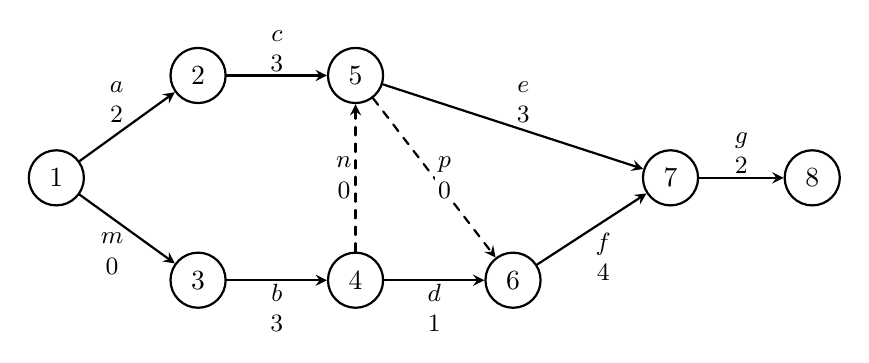
\begin{tikzpicture}[>=stealth,thick,line cap=round,line join=round,
  event/.style={circle,draw,minimum size=7mm,inner sep=0pt},
  activity/.style={font=\small,align=center,fill=white,inner sep=1pt}]
  \node[event] (v1) at (0,0) {1};
  \node[event] (v2) at (1.8,1.3) {2};
  \node[event] (v3) at (1.8,-1.3) {3};
  \node[event] (v4) at (3.8,-1.3) {4};
  \node[event] (v5) at (3.8,1.3) {5};
  \node[event] (v6) at (5.8,-1.3) {6};
  \node[event] (v7) at (7.8,0) {7};
  \node[event] (v8) at (9.6,0) {8};
  \draw[->] (v1) -- node[activity,above left] {$a$\\$2$} (v2);
  \draw[->] (v1) -- node[activity,below left] {$m$\\$0$} (v3);
  \draw[->] (v2) -- node[activity,above] {$c$\\$3$} (v5);
  \draw[->] (v3) -- node[activity,below] {$b$\\$3$} (v4);
  \draw[->,dashed] (v4) -- node[activity,left] {$n$\\$0$} (v5);
  \draw[->] (v4) -- node[activity,below] {$d$\\$1$} (v6);
  \draw[->,dashed] (v5) -- node[activity,right] {$p$\\$0$} (v6);
  \draw[->] (v5) -- node[activity,above right] {$e$\\$3$} (v7);
  \draw[->] (v6) -- node[activity,below right] {$f$\\$4$} (v7);
  \draw[->] (v7) -- node[activity,above] {$g$\\$2$} (v8);
\end{tikzpicture}
\end{center}
\nopagebreak[4]
\Needspace{4\baselineskip}
\textbf{解析}

由工序箭头约束，关键路径为$1\to2\to5\to6\to7\to8$，工时$2+3+0+4+2=11$天。其余完整路径不超过11天；虚箭头$n,p$工时均为0。

\gkanswer{答案：$11$ 天。}

\end{answer}
\begin{answer}
\gksolhead{7}{}

\textbf{题目}：

袋内装有大小相同的4个白球和3个黑球，从中任意摸出3个球，其中只有一个黑球的概率是 \gkblank{}。

\Needspace{4\baselineskip}
\textbf{解析}

超几何计数为 $\binom31\binom42/\binom73=18/35$。

\gkanswer{答案：$\dfrac{18}{35}$。}

\end{answer}
\begin{answer}
\gksolhead{8}{}

\textbf{题目}：

\Needspace{5\baselineskip}
函数
\nopagebreak[4]
\[
y=\begin{cases}
2x+3,&x\le 0,\\
x+3,&0<x\le1,\\
-x+5,&x>1
\end{cases}
\]
的最大值是 \gkblank{}。

\Needspace{4\baselineskip}
\textbf{解析}

分段函数在$x=1$处取值4；首段最大值3，末段对$x>1$有$-x+5<4$，故最大值4。

\gkanswer{答案：$4$。}

\end{answer}
\begin{answer}
\gksolhead{9}{}

\textbf{题目}：

设 $n$ 是一个自然数，$\left(1+\dfrac{x}{n}\right)^n$ 的展开式中 $x^3$ 的系数为 $\dfrac1{16}$，则 $n=$ \gkblank{}。

\Needspace{4\baselineskip}
\textbf{解析}

$x^3$系数 $\binom n3/n^3=1/16$，化为 $5n^2-24n+16=0$；自然数解为$n=4$。

\gkanswer{答案：$4$。}

\end{answer}
\begin{answer}
\gksolhead{10}{}

\textbf{题目}：

在数列 $\{a_n\}$ 和 $\{b_n\}$ 中，$a_1=2$，且对任意自然数 $n$，$3a_{n+1}-a_n=0$；$b_n$ 是 $a_n$ 与 $a_{n+1}$ 的等差中项，则 $\{b_n\}$ 的各项和是 \gkblank{}。

\Needspace{4\baselineskip}
\textbf{解析}

$a_n=2(1/3)^{n-1}$，$b_n=(a_n+a_{n+1})/2=(2/3)a_n$。故$\sum_{n=1}^\infty b_n=(2/3)\cdot 2/(1-1/3)=2$。

\gkanswer{答案：$2$。}

\end{answer}
\begin{answer}
\gksolhead{11}{}

\textbf{题目}：

与椭圆 $\dfrac{x^2}{49}+\dfrac{y^2}{24}=1$ 有相同焦点且以 $y=\pm\dfrac43x$ 为渐近线的双曲线方程是 \gkblank{}。

\Needspace{4\baselineskip}
\textbf{解析}

椭圆焦半距$c=\sqrt{49-24}=5$。双曲线渐近线斜率给$b/a=4/3$，且$c^2=a^2+b^2$，得$a=3,b=4$，方程为$\frac{x^2}{9}-\frac{y^2}{16}=1$。

\gkanswer{答案：$\dfrac{x^2}{9}-\dfrac{y^2}{16}=1$。}

\end{answer}
\begin{answer}
\gksolhead{12}{}

\textbf{题目}：

下列函数中，周期为 $\dfrac\pi2$ 的偶函数是\mbox{（　　）}

（A）$y=\sin4x$　（B）$y=\cos^22x-\sin^22x$　（C）$y=\operatorname{tg}2x$　（D）$y=\cos2x$

\Needspace{4\baselineskip}
\textbf{解析}

B项$\cos^22x-\sin^22x=\cos4x$，是偶函数，周期为$\pi/2$，选B。

\gkanswer{答案：B。}

\end{answer}
\begin{answer}
\gksolhead{13}{}

\textbf{题目}：

若 $0<a<1$，则函数 $y=\log_a(x+5)$ 的图象不过\mbox{（　　）}

（A）第一象限　（B）第二象限　（C）第三象限　（D）第四象限

\Needspace{4\baselineskip}
\textbf{解析}

定义域$x>-5$。当$-5<x<-4$时函数值为正且$x<0$，图象经过第二象限；当$-4<x<0$时函数值为负且$x<0$，经过第三象限；当$x>0$时函数值为负，经过第四象限。因此第一象限不经过，选A。

\gkanswer{答案：A。}

\end{answer}
\begin{answer}
\gksolhead{14}{}

\textbf{题目}：

在下列命题中，假命题是\mbox{（　　）}

（A）若平面 $\alpha$ 内的一条直线 $l$ 垂直于平面 $\beta$ 内的任一条直线，则 $\alpha\perp\beta$。

（B）若平面 $\alpha$ 内的任一直线平行于平面 $\beta$，则 $\alpha\parallel\beta$。

（C）若平面 $\alpha\perp\beta$，任取直线 $l\subset\alpha$，则有 $l\perp\beta$。

（D）若平面 $\alpha\parallel\beta$，任取直线 $l\subset\alpha$，则有 $l\parallel\beta$。

\Needspace{4\baselineskip}
\textbf{解析}

A为真：若$\alpha$内直线$l$垂直于$\beta$内任意直线，取$\beta$内两条相交直线，则$l$垂直于这两条相交直线，从而$l\perp\beta$，故$\alpha\perp\beta$。B为真：若$\alpha$与$\beta$相交，则交线是$\alpha$内一条不平行于$\beta$的直线；若两平面重合，$\alpha$内的直线也都不平行于$\beta$，均与前提矛盾，所以两平面没有公共点，即$\alpha\parallel\beta$。C为假：当$\alpha\perp\beta$时，两平面的交线$l=\alpha\cap\beta$属于$\alpha$，但$l\subset\beta$，并不垂直于$\beta$。D为真：若$\alpha\parallel\beta$，则$\alpha$内任一直线都不与$\beta$相交，故该直线平行于$\beta$。因此选C。

\gkanswer{答案：C。}

\end{answer}
\begin{answer}
\gksolhead{15}{}

\textbf{题目}：

设全集为 $\mathbb R$，$A=\{x\mid x^2-5x-6>0\}$，$B=\{x\mid |x-5|<a\}$（$a$为常数），且 $11\in B$，则\mbox{（　　）}

（A）$\overline A\cup B=\mathbb R$　（B）$A\cup\overline B=\mathbb R$　（C）$\overline A\cup\overline B=\mathbb R$　（D）$A\cup B=\mathbb R$

\Needspace{4\baselineskip}
\textbf{解析}

原页条件为$11\in B$，即$|11-5|<a$，所以$a>6$。解不等式得$A=(-\infty,-1)\cup(6,+\infty)$、$\overline A=[-1,6]$，而$B=(5-a,5+a)$满足$5-a<-1$、$5+a>11>6$，故$\overline A\subset B$，D项$A\cup B=\mathbb R$成立。其余选项均不成立：A项要求无界集$A\subset B$；B项在$x=0$处为假；C项在$x=7$处为假。故D是唯一正确项，与卷内答案表一致。此前误读成$1\in B$导致的ISSUE-1115已解决；本稿仍不将扫描件答案认证为官方答案。

\gkanswer{答案：D（原页核读 $11\in B$）。}

\end{answer}
\begin{answer}
\gksolhead{16}{}

\textbf{题目}：

设 $a,b,c$ 分别是 $\triangle ABC$ 中 $\angle A,\angle B,\angle C$ 所对边的边长，则直线
$\sin A\,x+ay+c=0$ 与 $bx-\sin B\,y+\sin C=0$ 的位置关系是\mbox{（　　）}

（A）平行　（B）重合　（C）垂直　（D）相交但不垂直

\Needspace{4\baselineskip}
\textbf{解析}

由正弦定理，$\sin A=a/(2R)$、$\sin B=b/(2R)$。两直线法向量可分别写为$(a/(2R),a)$、$(b,-b/(2R))$，点积为$ab/(2R)-ab/(2R)=0$，故两直线垂直，选C。

\gkanswer{答案：C。}

\end{answer}
\begin{answer}
\gksolhead{17}{}

\textbf{题目}（8分）：

设 $\alpha$ 是第二象限角，$\sin\alpha=\dfrac35$，求 $\sin\left(\dfrac{37\pi}{6}-2\alpha\right)$ 的值。

\Needspace{4\baselineskip}
\textbf{解析}

\Needspace{5\baselineskip}
因$\alpha$在第二象限且$\sin\alpha=3/5$，故$\cos\alpha=-4/5$。于是
\nopagebreak[4]
\[
\sin2\alpha=-\frac{24}{25},\qquad \cos2\alpha=\frac7{25}.
\]
\Needspace{5\baselineskip}
又$37\pi/6=6\pi+\pi/6$，所以
\nopagebreak[4]
\[
\sin\left(\frac{37\pi}{6}-2\alpha\right)
=\sin\left(\frac\pi6-2\alpha\right)
=\frac12\cdot\frac7{25}-\frac{\sqrt3}{2}\cdot\left(-\frac{24}{25}\right)
=\frac{7+24\sqrt3}{50}.
\]

\gkanswer{答案：$\sin\left(\dfrac{37\pi}{6}-2\alpha\right)=\dfrac{7+24\sqrt3}{50}$。}

\end{answer}
\begin{answer}
\gksolhead{18}{}

\textbf{题目}（12分）：

已知复数 $z_1$ 满足 $(z_1-2)i=1+i$，复数 $z_2$ 的虚部为 $2$，且 $z_1\cdot z_2$ 是实数，求复数 $z_2$ 的模。

\Needspace{4\baselineskip}
\textbf{解析}

\Needspace{5\baselineskip}
$(z_1-2)i=1+i$，故$z_1=3-i$。令$z_2=t+2i$（$t\in\mathbb R$），则
\nopagebreak[4]
\[
z_1z_2=(3-i)(t+2i)=(3t+2)+(6-t)i.
\]
乘积为实数给出$t=6$，因此$z_2=6+2i$、$|z_2|=2\sqrt{10}$。

\gkanswer{答案：$z_2=6+2i$，$|z_2|=2\sqrt{10}$。}

\end{answer}
\begin{answer}
\gksolhead{19}{}

\textbf{题目}（16分）：

本题共两个小题，第（1）小题8分，第（2）小题8分。直四棱柱 $ABCD\text{-}A_1B_1C_1D_1$ 的高为 $6$，底面是边长为 $4$、$\angle DAB=60^\circ$ 的菱形，$AC$ 与 $BD$ 相交于 $O$，$A_1C_1$ 与 $B_1D_1$ 相交于 $O_1$，$E$ 是 $O_1A$ 的中点。

（1）求二面角 $O_1\text{-}BC\text{-}D$ 的大小（用反三角函数表示）；

（2）分别以射线 $OA,OB,OO_1$ 为 $x$轴、$y$轴、$z$轴的正半轴建立空间直角坐标系，求点 $B_1,D_1,E$ 的坐标，并求异面直线 $OB_1$ 与 $D_1E$ 所成角的大小（用反三角函数表示）。
\nopagebreak[4]
\begin{center}% 1998 上海文科第19题：直四棱柱、底面菱形与对角线/辅助线关系；示意图不按比例。
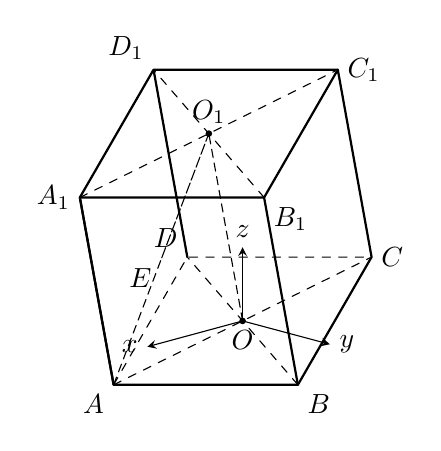
\begin{tikzpicture}[x=0.78cm,y=0.78cm,>=stealth,line cap=round,line join=round]
  \coordinate (A)  at (0,0);
  \coordinate (B)  at (3,0);
  \coordinate (C)  at (4.2,2.08);
  \coordinate (D)  at (1.2,2.08);
  \coordinate (A1) at (-0.55,3.05);
  \coordinate (B1) at (2.45,3.05);
  \coordinate (C1) at (3.65,5.13);
  \coordinate (D1) at (0.65,5.13);
  \coordinate (O)  at (2.1,1.04);
  \coordinate (O1) at (1.55,4.09);
  \coordinate (E)  at (0.775,2.045);
  % 棱柱棱；遮挡部分使用虚线。
  \draw[thick] (A)--(B)--(C)--(C1)--(B1)--(A1)--cycle;
  \draw[thick] (A1)--(D1)--(C1) (D1)--(D);
  \draw[thick] (A)--(A1) (B)--(B1);
  \draw[dashed] (A)--(D)--(C) (D)--(D1);
  % 上下底面对角线及辅助连线。
  \draw[dashed] (A)--(C) (B)--(D) (A1)--(C1) (B1)--(D1);
  \draw[densely dashed] (A)--(O1) (O1)--(E) (O)--(O1);
  \fill (O) circle (1.2pt);
  \fill (O1) circle (1.2pt);
  \node[below left] at (A) {$A$};
  \node[below right] at (B) {$B$};
  \node[right] at (C) {$C$};
  \node[above left] at (D) {$D$};
  \node[left] at (A1) {$A_1$};
  \node[below right] at (B1) {$B_1$};
  \node[right] at (C1) {$C_1$};
  \node[above left] at (D1) {$D_1$};
  \node[below] at (O) {$O$};
  \node[above] at (O1) {$O_1$};
  \node[below left] at (E) {$E$};
  % 坐标轴方向与题面指定一致，仅表示方向。
  \draw[->] (O) -- ++(-1.55,-0.42) node[left] {$x$};
  \draw[->] (O) -- ++(1.42,-0.38) node[right] {$y$};
  \draw[->] (O) -- ++(0,1.2) node[above] {$z$};
\end{tikzpicture}
\end{center}
\nopagebreak[4]
\Needspace{4\baselineskip}
\textbf{解析}

（1）底面菱形的对角线互相垂直且平分，故$OA=OC=2\sqrt3$、$OB=OD=2$。令$F$为$O$到$BC$的垂足，则$[OBC]=\frac12 OB\cdot OC=2\sqrt3$，从而$OF=2[OBC]/BC=\sqrt3$。棱柱高$OO_1=6$且垂直底面，所以$\triangle OO_1F$在$O$处直角，所求二面角的平面角为$\angle O_1FO$，其正切为$6/\sqrt3=2\sqrt3$。角为$\arctan(2\sqrt3)$。

\Needspace{5\baselineskip}
（2）按题设坐标轴，$O(0,0,0)$、$B_1(0,2,6)$、$D_1(0,-2,6)$、$E(\sqrt3,0,3)$。于是
\nopagebreak[4]
\[
\overrightarrow{OB_1}=(0,2,6),\quad\overrightarrow{D_1E}=(\sqrt3,2,-3),\quad
\overrightarrow{OB_1}\cdot\overrightarrow{D_1E}=-14,
\]
\Needspace{5\baselineskip}
且$|OB_1|=2\sqrt{10}$、$|D_1E|=4$。固定这两个向量方向时夹角余弦为$-7\sqrt{10}/40$，对应约$123.6^\circ$的有向向量钝角；两条无向直线的通常夹角取锐角，故
\nopagebreak[4]
\[
\theta=\arccos\!\left(\frac{7\sqrt{10}}{40}\right).
\]
扫描件解答先列出上述负余弦，随后明确给出异面直线所成角为$\arccos(7\sqrt{10}/40)\approx56.4^\circ$，与本文按标准直线角定义所得结论一致。

\gkanswer{答案：（1）二面角 $O_1\text{-}BC\text{-}D$ 的大小为 $\arctan(2\sqrt3)$；（2）异面直线 $OB_1$ 与 $D_1E$ 所成角为 $\arccos\dfrac{7\sqrt{10}}{40}$。}

\end{answer}
\begin{answer}
\gksolhead{20}{}

\textbf{题目}（16分）：

本题共两个小题，第（1）小题6分，第（2）小题10分。

（1）设动点 $M$ 到定点 $D(2,0)$ 的距离与到 $y$ 轴的距离相等，求点 $M$ 的轨迹 $C$ 的方程；

（2）过点 $D(2,0)$ 的直线 $l$ 交上述轨迹 $C$ 于 $P,Q$ 两点，点 $E$ 的坐标是 $(1,0)$。若 $\triangle EPQ$ 的面积为 $4$，求直线 $l$ 的倾斜角 $\alpha$。

\Needspace{4\baselineskip}
\textbf{解析}

（1）设$M=(x,y)$。到$D(2,0)$的距离等于到$y$轴的距离，故$\sqrt{(x-2)^2+y^2}=|x|$。平方并化简得$y^2=4(x-1)$。

\Needspace{5\baselineskip}
（2）先检查竖直线$l:x=2$：它与抛物线交于$P=(2,2)$、$Q=(2,-2)$，故$|PQ|=4$；点$E=(1,0)$到$l$的距离为$1$，三角形面积为$2\ne4$，所以竖直线不是解。对其余直线设$l:y=k(x-2)$。若$k=0$，直线与抛物线只有顶点一个交点，不符合有$P,Q$两交点，故$k\ne0$。以交点纵坐标$y_1,y_2$表示，则代入抛物线得到
\nopagebreak[4]
\[
y^2-\frac4k y-4=0,
\]
\Needspace{5\baselineskip}
由韦达定理，$y_1+y_2=4/k$、$y_1y_2=-4$，所以
\nopagebreak[4]
\[
|y_1-y_2|=\sqrt{(y_1+y_2)^2-4y_1y_2}=\frac{4\sqrt{k^2+1}}{|k|}.
\]
\Needspace{5\baselineskip}
从而$|PQ|=\sqrt{1+1/k^2}|y_1-y_2|=4(k^2+1)/k^2$。点$E(1,0)$到直线$kx-y-2k=0$的距离为$|k|/\sqrt{k^2+1}$，故
\nopagebreak[4]
\[
S_{\triangle EPQ}=\frac12|PQ|\,d=\frac{2\sqrt{k^2+1}}{|k|}=4.
\]
解得$k^2=1/3$。按倾斜角$\alpha\in[0,\pi)$，$k=\tan\alpha$，所以$\alpha=\pi/6$或$5\pi/6$。
\nopagebreak[4]
\begin{center}% 1998 上海文科第20题：抛物线、焦点D、点E及过D的割线关系示意；不按比例、不编码题设未给的精确斜率。
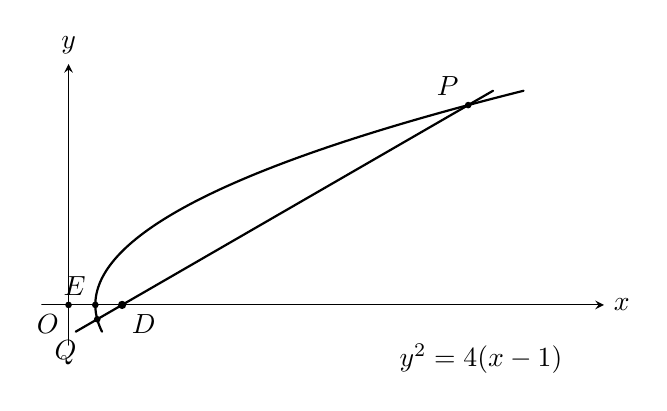
\begin{tikzpicture}[x=0.34cm,y=0.34cm,>=stealth,line cap=round,line join=round]
  \draw[->] (-1,0)--(20,0) node[right] {$x$};
  \draw[->] (0,-1.5)--(0,9) node[above] {$y$};
  \draw[thick,domain=-1:8,samples=100] plot ({1+\x*\x/4},{\x});
  % 示出一条过焦点D的示意割线(斜率1/sqrt(3))；非源卷坐标，不按比例。
  \draw[thick,domain=-1:8,variable=\y] plot ({2+sqrt(3)*\y},{\y});
  \coordinate (P) at ({2+sqrt(3)*(2*sqrt(3)+4)},{2*sqrt(3)+4});
  \coordinate (Q) at ({2+sqrt(3)*(2*sqrt(3)-4)},{2*sqrt(3)-4});
  \fill (0,0) circle (1.2pt) node[below left] {$O$};
  \fill (1,0) circle (1.2pt) node[above left] {$E$};
  \fill (2,0) circle (1.5pt) node[below right] {$D$};
  \fill (P) circle (1.2pt) node[above left] {$P$};
  \fill (Q) circle (1.2pt) node[below left=4pt] {$Q$};
  \node[below right] at (12,-1.1) {$y^2=4(x-1)$};
\end{tikzpicture}
\end{center}
\nopagebreak[4]
\gkanswer{答案：（1）$y^2=4(x-1)$；（2）$\alpha=\dfrac\pi6$ 或 $\dfrac{5\pi}6$。}

\end{answer}
\begin{answer}
\gksolhead{21}{}

\textbf{题目}（16分）：

\Needspace{5\baselineskip}
本题共三个小题，第（1）小题6分，第（2）小题7分，第（3）小题3分。设某物体一天中的温度 $T$ 是时间 $t$ 的函数：
\nopagebreak[4]
\[
T(t)=at^3+bt^2+ct+d\quad(a\ne0),
\]
其中温度单位是摄氏度，时间单位是小时，$t=0$ 表示12:00，$t$ 取正值表示12:00以后。若测得该物体在8:00的温度为 $8^\circ\mathrm C$，12:00的温度为 $60^\circ\mathrm C$，13:00的温度为 $58^\circ\mathrm C$，且已知该物体的温度在8:00和16:00有相同的变化率。

（1）写出该物体的温度 $T$ 关于时间 $t$ 的函数关系式；

（2）该物体在10:00到14:00这段时间中（包括10:00和14:00），何时温度最高？并求出最高温度；

（3）如果规定一个函数 $f(x)$ 在 $[x_1,x_2]$（$x_1<x_2$）上函数值的平均为 $\dfrac1{x_2-x_1}\int_{x_1}^{x_2}f(x)\,dx$，求该物体在8:00到16:00这段时间内的平均温度。

\Needspace{4\baselineskip}
\textbf{解析}

\Needspace{5\baselineskip}
由$T(0)=60$得$d=60$。其余三个条件为$T(-4)=8$、$T(1)=58$和$T'(-4)=T'(4)$。由$T'(t)=3at^2+2bt+c$，
\nopagebreak[4]
\[
T'(-4)=48a-8b+c,\qquad T'(4)=48a+8b+c,
\]
\Needspace{5\baselineskip}
故$b=0$。两个温度条件于是化为
\nopagebreak[4]
\[
-64a-4c=-52,\qquad a+c=-2,
\]
\Needspace{5\baselineskip}
即$16a+c=13$和$a+c=-2$，解得$a=1,c=-3$，所以$T(t)=t^3-3t+60$。在$[-2,2]$上，$T'(t)=3(t-1)(t+1)$，故函数依次在$[-2,-1]$递增、$[-1,1]$递减、$[1,2]$递增。端点和驻点处的函数值为$T(-2)=T(1)=58$、$T(-1)=T(2)=62$，所以11:00和14:00均达到最高温度$62^\circ\mathrm C$。平均温度为
\nopagebreak[4]
\[
\frac18\int_{-4}^{4}(t^3-3t+60)\,dt=60^\circ\mathrm C,
\]
因为两个奇函数项在对称区间上的积分为零。

\gkanswer{答案：$T(t)=t^3-3t+60$；11:00 与 14:00 均为最高温度 $62^\circ\mathrm C$；8:00–16:00 平均温度 $60^\circ\mathrm C$。}

\end{answer}
\begin{answer}
\gksolhead{22}{}

\textbf{题目}（18分）：

\Needspace{5\baselineskip}
本题共三个小题，第（1）小题4分，第（2）小题8分，第（3）小题6分。若 $A_n$ 和 $B_n$ 分别表示数列 $\{a_n\}$ 和 $\{b_n\}$ 前 $n$ 项的和，对任意正整数 $n$，
\nopagebreak[4]
\[
a_n=-\frac{2n+3}{2},\qquad 4B_n-12A_n=13n.
\]

（1）求数列 $\{b_n\}$ 的通项公式；

\Needspace{5\baselineskip}
（2）设有抛物线列 $C_1,C_2,\ldots,C_n,\ldots$，抛物线 $C_n:y=a(x-a_n)^2+b_n\ (n\in\mathbb N)$ 通过点 $D_n(0,n^2+1)$。过点 $D_n$ 与抛物线 $C_n$ 相切的直线斜率为 $k_n$，求极限
\nopagebreak[4]
\[
\lim_{n\to\infty}\frac{k_1+k_2+\cdots+k_n}{a_nb_n};
\]

（3）设集合 $X=\{x\mid x=2a_n,\ n\in\mathbb N\}$，$Y=\{y\mid y=4b_n,\ n\in\mathbb N\}$。把 $X\cap Y$ 中小于 $-100$ 的元素从大到小排列构成数列 $\{c_n\}$，求 $c_n$ 的通项公式。

\Needspace{4\baselineskip}
\textbf{解析}

（1）对$n\ge2$，相邻两项前$n$项和关系相减得$4b_n-12a_n=13$。代入$a_n=-(2n+3)/2$，得$b_n=-(12n+5)/4$。$n=1$时原关系给$4b_1-12a_1=13$，也得到$b_1=-17/4$，与通项一致。

\Needspace{5\baselineskip}
（2）把题面的$a$视为对所有$n$固定的二次项系数（原题未另作定义）；由抛物线通过$D_n(0,n^2+1)$，有$n^2+1=a a_n^2+b_n$。代入$a_n=-(2n+3)/2$、$b_n=-(12n+5)/4$并整理得$(a-1)(2n+3)^2=0$，故固定系数$a=1$。因此
\nopagebreak[4]
\[
y=\left(x+\frac{2n+3}{2}\right)^2-\frac{12n+5}{4}
=x^2+(2n+3)x+n^2+1,
\]
在$D_n$处的切线斜率$k_n=2n+3$。所以$\sum_{i=1}^{n}k_i=n^2+4n$，而$a_nb_n=(2n+3)(12n+5)/8$，所求极限为$1/3$。

（3）题设仅对正整数$n$定义$a_n,b_n$，集合指标沿用题设数列项的正整数定义域，不另加未定义的$n=0$项。于是$X=\{-5,-7,-9,\ldots\}$，$Y=\{-17,-29,-41,\ldots\}$。对任意$n\in\mathbb N^+$，$4b_n=-12n-5=2a_{6n+1}$，故$Y\subseteq X$且$X\cap Y=Y$。条件$4b_n=-(12n+5)<-100$等价于$n>95/12$，即$n\ge8$。从大到小排列时首项为$4b_8=-101$，公差$-12$，故$c_n=-101-12(n-1)=-12n-89$。

\gkanswer{答案：（1）$b_n=-\dfrac{12n+5}{4}$；（2）$\lim\limits_{n\to\infty}\dfrac{k_1+k_2+\cdots+k_n}{a_nb_n}=\dfrac13$；（3）$c_n=-12n-89$。}

\end{answer}